\chapter{The Standard Model of particle physics}
\chaptermark{The Standard Model of particle physics}  
\thispagestyle{plain}  % First page has default style
\pagestyle{chapterpages}
\label{Section:Chapter1}
The \ac{SM} of particle physics~\cite{Glashow_StandardModel_1,Weinberg_StandardModel_1,StandardModel_3,Standard_Model4} is our current best theoretical framework underpinning our understanding of the subatomic world, providing a description of fundamental elementary particles and their interactions via the electromagnetic force, weak nuclear force and the strong nuclear force. The fourth fundamental force of nature, Gravity, is absent from the SM, highlighting one of its key limitations. However, in high-energy physics experiments, where the interactions of subatomic particles are being studied, the omission of gravity is considered a safe simplification. Extremely powerful predictions have emerged from this theoretical framework, with its greatest accomplishments being the prediction~\cite{Higgs_1} and subsequent discovery of the Higgs boson in 2012~\cite{Higgs_ATLAS,Higgs_CMS}. Despite its success, the Standard Model has its limitations. Along with the absence of gravity, it leaves several fundamental questions unanswered, such as the nature of neutrino oscillations~\cite{Neutrino_Oscillations}, the existence of dark matter~\cite{DarkMatter}, the hierarchy problem~\cite{HierarchyProblem}, and the matter-antimatter asymmetry in the universe~\cite{MatterAntimatter}, driving the field to look for explanations beyond the SM. In the pursue of \ac{BSM} physics, a deep understanding of the SM theory is crucial. The goal of this chapter is to establish the base foundation for this work, the SM, by exploring the fundamental blocks of the theory, including its particle content, interactions, and the Higgs mechanism.

\section{Particle content and fundamental interactions}
\label{Section:Particle content and fundamental interactions}
Built upon the theoretical framework of QFT, the Standard Model (SM) is a renormalisable theory in which the physical particles observed in nature, namely fermions, emerge as quantised excitations of underlying relativistic fields. Their interactions are mediated by force carriers, specifically vector bosons, and together these two groups of particles constitute the particle content of the SM, as shown in Fig.~\ref{Figure:Introduction_1}.

\begin{figure}[h]
\centering
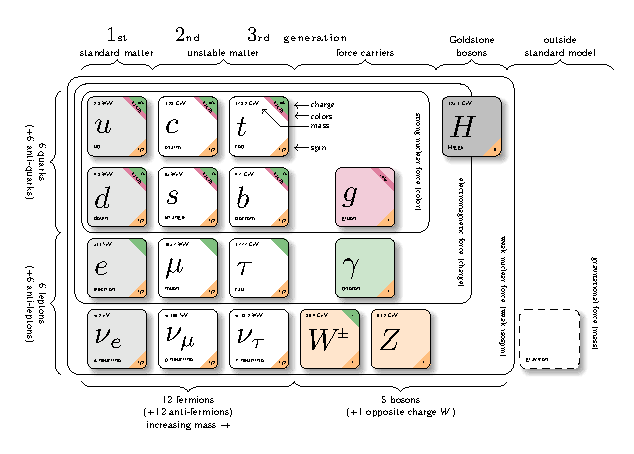
\includegraphics[width= 0.9\textwidth]{Figures/Introduction/Particles.pdf}
\caption{Diagram of the particle content of the SM. For each fundamental particle, the charges, colour and spin quantum numbers are available. The measured masses for all fermions and gauge bosons are taken from Ref.~\cite{ParticleMasses} with the exception of the Higgs mass which is taken from Ref.~\cite{Higgs_Mass}.}
\label{Figure:Introduction_1}
\end{figure}

Within the SM, fermions serve as the fundamental constituents of all observable matter. These elementary, non-composite, spin-1/2 particles are organised into three distinct generations, with each fermion paired with an antiparticle that exhibits quantum numbers precisely opposite in sign with the exception of mass and spin, which remain identical. As shown in Fig.~\ref{Figure:Introduction_1}, fermions are further divided into quarks and leptons. 

The leptonic sector consists of three charged leptons (electron, muon, tau) and three electrically neutral neutrinos (electron neutrino, muon neutrino, tau neutrino). The quark sector, on the other hand, comprises of six quark flavours; up, down, charm, strange, top and bottom. Within the first generation, the electron and electron neutrino represent the leptons, while the up and down quarks form the quark sector. Although fundamental quantum numbers remain identical across generations, the mass spectrum exhibits a strong hierarchy, with the third generation being significantly heavier than the first.

A key distinction between leptons and quarks lies in their participation in strong interactions. Unlike leptons, quarks possess an additional quantum number known as colour charge, enabling their interactions via the strong force mediated by massless gluons ($g$). In addition to the strong interaction, charged leptons and quarks interact electromagnetically due to their electric charge with massless photons ($\gamma$) acting as the mediators of the force. Conversely, neutrinos, being electrically neutral, do not participate in electromagnetic interactions. All fermions, including neutrinos, interact via the weak interaction which occurs via the exchange of massive vector bosons: W ($\text{W}^\pm$) bosons and Z boson. These fundamental interactions are explored in more detail in the following section.

\section{Foundation of the fundamental interactions}
\label{Section:Chapter1_FundamentalInteractions}

In the core of QFT and the SM lies the principle of symmetry, with the Lagrangian density serving as the starting point of describing fundamental interactions. Fundamental laws are closely tied to symmetries. N\"{o}ether's theorem shows that a conservation law is implied by the invariance of a Lagrangian under a continuous transformation (symmetry). A striking example of the deep connection between fundamental interactions and symmetry principles is the conversation of angular momentum, defined by a Lagrangian which is invariant under rotational transformations. 

The SM is a gauge theory built on the principle of local gauge invariance \ie the Lagrangian is invariant under local phase transformations. In contrast to global phase transformations, such transformations shift the phase of the field ($\psi(x)$) as a function of the spacetime coordinates; $\psi(x) \rightarrow e^{iq\theta(x)} \psi(x)$. The introduction of the gauge boson fields mediating fermion interactions is a direct consequence of imposing this invariance. Alone a local phase transformation would break the invariance of the SM Lagrangian which is restored by the introduction of the gauge boson fields.

\subsection{Quantum Electrodynamics}

The QFT of electromagnetism, known as \ac{QED}, describes the interactions between charged fermions through the exchanged of photons. Remarkably, the entire framework of QED emerges beautifully from a single guiding principle; the requirement that the QED Lagrangian remains invariant under local U(1) gauge transformations. The foundation of QED begins with the Dirac equation \cite{DiracEquation} which describes the equations of motion for spin-$\frac{1}{2}$ fermion fields,

\begin{equation}
    \mathcal{L}_{Dirac} = \overline{\psi}(i\gamma^\mu \partial_\mu - m_{\psi}) \psi
\label{Equation:Dirac}
\end{equation}

where $\psi$ and its adjoint $\overline{\psi}$ are the fermion fields expressed as four-component Dirac spinors while the quantity $\gamma^\mu$ represents the Dirac gamma matrices. Finally, $m_{\psi}$ represents the mass of the fermion.

As briefly discussed in Section~\ref{Section:Chapter1_FundamentalInteractions}, under a local U(1) gauge transformation, the fermion field transforms as $\psi(x) \rightarrow e^{iq\theta(x)} \psi(x)$ and this breaks the local gauge invariance of the Lagrangian. Under this transformation, the Dirac equation (Equation~\ref{Equation:Dirac} becomes

\begin{equation}
    U(1) \rightarrow \mathcal{L}_{Dirac}^{\prime} = \mathcal{L}_{Dirac} - q\overline{\psi}(\partial_\mu\theta(x))\psi
\label{Equation:Dirac(U1)}
\end{equation}

To restore local gauge invariance, the derivative $\partial_\mu$ is replaced with the covariant derivative $D_\mu$,

\begin{equation}
    \partial_\mu \rightarrow D_\mu = \partial_\mu + iqA_\mu
\end{equation}

where $A_\mu$ is a new field. The problematic term in Equation~\ref{Equation:Dirac(U1)} can be cancelled out provided that the new field transforms as

\begin{equation}
    U(1) \rightarrow A_\mu^{\prime} = A_\mu - \partial_\mu \theta(x) 
\end{equation}

Therefore, imposing a U(1) local gauge invariance on the Lagrangian has forced the existence of a photon field, $A_\mu$, with well-defined gauge transformation properties. The local gauge-invariant Lagrangian for a spin-$\frac{1}{2}$ becomes

\begin{equation}
    \mathcal{L}_{Dirac} = \overline{\psi}(i\gamma^\mu \partial_\mu - m_{\psi}) \psi - q\overline{\psi}\gamma^\mu A_\mu\psi
\label{Equation:Dirac_GaugeInvariant}
\end{equation}

The additional term in the Lagrangian (Equation~\ref{Equation:Dirac_GaugeInvariant}) encapsulates the electromagnetic interaction between charged fermions and photons. The strength of this coupling is given by $q = |e|Q$, where e denotes the fundamental unit of electric charge, and Q represents the dimensionless charge of the fermion field $\psi$ relative to e. By N\"{o}ether's theorem, electric charge corresponds to the conserved quantity associated with local U(1) gauge symmetry, once again reinforcing the deep connection between symmetry and conservation laws in QFT. The final component necessary to complete the QED Lagrangian is the gauge-invariant kinetic term for the massless spin-1 field, described by the field strength tensor $F_{\mu\nu}$. Incorporating this, the total QED Lagrangian takes the form,

\begin{equation}
    \mathcal{L}_{QED} = \overline{\psi}(i\gamma^\mu \partial_\mu - m_{\psi}) \psi - q\overline{\psi}\gamma^\mu A_\mu\psi - \frac{1}{4}F_{\mu\nu}F^{\mu\nu}
\label{Equation:Dirac_GaugeInvariant}
\end{equation}

\subsection{Quantum Chromodynamics}

The QFT describing the strong interaction is known as \ac{QCD}. QCD governs the dynamics of quarks and gluons, and it is formulated as a non-Abelian gauge theory under the local $SU(3)_C$ symmetry group. In contrast to QED which applies universally on all charged particles, the gauge symmetry of QCD only applies on fields that carry colour charge, as denoted by the subscript C.

Unlike the Abelian U(1) symmetry of QED which involves a single generator, the SU(3) symmetry group is represent by eight generators, $T^a$. To ensure local $SU(3)_C$ gauge invariance, the derivative $\partial_\mu$ is replaced with the covariant derivative expressed in terms of the generators as,

\begin{equation}
    \partial_\mu \rightarrow D_\mu = \partial_\mu + ig_sG^{a}_{\mu}T^{a}
\end{equation}

where $G^{a}_{\mu}$ represent the eight new fields, corresponding to the eight massless gluons mediating the strong interaction and $g_s$ encodes the coupling strength of the interaction. The full QCD Lagrangian can then be expressed as

\begin{equation} 
\mathcal{L}_{QCD} = \sum_{f}\overline{\psi_f}(i\gamma^\mu D_\mu - m_f)\psi_f - \frac{1}{4} G^{\mu\nu}_{a}G^{a}_{\mu\nu}
\end{equation}

where $\psi_f$ represents the quark field (spinor) for the j-th flavour. Once again according to N\"{o}ether's theorem, colour charge corresponds to the conserved quantity associated with local $SU(3)_C$ gauge symmetry.

Unlike QED, the kinetic (gauge term) in the Lagrangian includes additional terms representing the self-interactions of the gauge bosons. This is a direct consequence of the generators of SU(3) not commuting ([$T^a,T^b$] = $if^{abc}T^c$), allowing gluons themselves to carry colour charge. The quantity $f^{abc}$ is known as the structure constants of the symmetry group. This gluon self-interaction property modifies the strength of the interaction ($\alpha_{S}$) causing it to decrease as a function of the interaction energy scale, hence $\alpha_{S}$ is referred to as a running coupling constant.

An important consequence of this, is asymptotic freedom~\cite{AsymptoticFreedom_1,AsymptoticFreedom_2}, where at very high energies (short distances), such as the deep scattering energies at the LHC, $\alpha_{S}$ decreases approaching zero. In this scenario, quarks and gluons behave as quasi-free particles within the protons and neutrons, , allowing perturbative QCD to accurately describe their interactions. However, at low energies, the strong coupling grows large, making QCD non-perturbative. In this regime, quarks and gluons are not found as free particles but instead form bound, color-neutral states known as hadrons. This phenomenon, known as color confinement, ensures that isolated color-charged particles do not exist in nature; only hadrons are observed.

As a consequence of colour confinement, in high-energy collisions, high-energy quarks and gluons are observed as jets~\cite{Hadronisation_Jets} of colourless particles formed through a process known as hadronisation. In the context of proton-proton (pp) collisions, highly energetic partons fly away from the interaction point. As the partons separate, the colour field between them partons can be thought as if it is being squeezed in a tube, with the energy in the field becoming increasingly larger with distance. Once that energy becomes sufficient a new quark-antiquark pair is produced, separating the colour field into smaller segments. Eventually the formation of colourless hadrons occurs when the quark-antiquark pairs have sufficiently low energy. This resulting cascade of collimated hadrons forms what is observed as a jet.

\subsection{Electroweak theory}

In the 1960s, Glashow~\cite{Glashow}, Salam~\cite{Salam} and Weinberg~\cite{Weinberg} discovered that a unified picture of the electromagnetic and weak interactions could be constructed. Their proposal was to develop the electroweak theory incorporating the characteristics of both interactions by associating them with the $SU(2)_{L}$ $\otimes$ $U(1)_{Y}$ symmetry group,

\begin{equation}
    SU(2)_L \otimes U(1)_Y \rightarrow \mathcal{L}^{\prime}_{EW} = \mathcal{L}_{EW}
\end{equation}

where L denotes the left-handed nature of the weak interaction under $SU(2)_L$, and Y represents the weak hypercharge associated with the $U(1)_Y$ gauge symmetry. To ensure that the electroweak Lagrangian is under local transformations of this symmetry group, the covariant derivative is written as

\begin{equation}
    D_\mu = \partial_\mu + \underbrace{g^{\prime}B^i_\mu Y}_{U(1)_Y} + \underbrace{\frac{i}{2}gW^i_\mu\sigma^i}_{SU(2)_L}
\end{equation}

where Y is the single generator of the $U(1)_Y$ gauge group, associated with the gauge boson field, $B_\mu$. While the three generators of $SU(2)_L$ are represented by the 2 x 2 Pauli-spin matrices ($\sigma^i$), associated with the three gauge boson fields, $W^i_\mu$. The coupling strengths of the interactions are represented by $g$ and $g^{\prime}$ respectively. The conserved charges corresponding to these gauge symmetries are the weak isospin component, $I_3$, for $SU(2)_L$ and the weak hypercharge, Y, for $U(1)_Y$.

By imposing gauge invariance under the electroweak symmetry group, four gauge fields arise: the three weak isospin fields, $W_{\mu}^{(i)}$ (i=1,2,3), and the weak hypercharge field, $B_{\mu}$. These gauge fields can be expressed in terms of the physical bosons as,

\begin{equation}
\begin{array}{c}
A_{\mu} = + B_{\mu} \cos{\theta_{W}} + W_{\mu}^{(3)} \sin{\theta_{W}}, \\
Z_{\mu} = - B_{\mu} \sin{\theta_{W}} + W_{\mu}^{(3)} \cos{\theta_{W}}, \\
W_{\mu}^{\pm} = \frac{1}{\sqrt{2}} (W_{\mu}^{(1)} \mp iW_{\mu}^{(2)}),
\end{array}
\label{Equation:Introduction_PhysicalGaugeFields}
\end{equation}

where $\theta_{W}$, the weak mixing angle, quantifies the mixing between the weak isospin and hypercharge gauge fields. It is related to the weak and electromagnetic coupling constants, $g$ and $g^{\prime}$, by

\begin{equation}
    \theta_W = \text{arctan}(\frac{g^{\prime}}{g})
\end{equation}

As discussed earlier in Section~\ref{Section:Particle content and fundamental interactions}, all fermions interact via the weak interaction. A key feature of the weak interaction is its violating of parity symmetry. This means that the weak interaction exhibits a different behavior under spatial translations. Using chiral operators, $P_{L/R}$, the fermion spinor fields ($u$) can be decomposed into left-handed ($u_{L}$) and right-handed ($u_{R}$) chiral components. 

\begin{equation}
    P_{L/R} = \frac{1}{2}(1\mp \gamma^5) \quad ,\quad \gamma^5 = \gamma^0\gamma^1\gamma^2\gamma^3
\end{equation}

This is engraved into the EW theory by only allowing interactions between left-handed fermions (right-handed anti-fermions) and the weak isospin fields, $W_{\mu}^{(i)}$. In this representation under $SU(2)_L$ transformations, the left-handed components of the fermion fields transform as doublets while the right-handed components transform as singlets. 

This structure of the EW theory naturally leads to a relationship between the weak isospin, weak hypercharge and electric charge.

\begin{equation}
    Q = I_3 + \frac{Y}{2}
\end{equation}

where this equation beautifully encapsulates how the EW symmetry unifies the electromagnetic and weak interactions, allowing for a calculation of the charge of all fundamental particles.

Despite, beautifully unifying the electromagnetic and weak interactions into a single theory, a fundamental issue persists because of non-zero mass measurements of the W and Z bosons~\cite{W_Z_MassMeasurements_1,W_Z_MassMeasurements_2}. This is clearly omitted from the EW Lagrangian as the inclusion of the required terms would break the underlying gauge symmetry. Mass terms of the form ${m_{W}^2 W_{\mu}^{-} W^{+\mu}}$ and $\frac{1}{2} m_{Z}^{2} Z_{\mu} Z^{\mu}$ are not invariant under the $SU(2)_{L}$ $\otimes$ $U(1)_{Y}$ symmetry group. This extends also to fermions with mass terms of the form, $m\overline{\psi}\psi = m(\overline{\psi}_{R}\psi_{L} + \overline{\psi}_{L}\psi_{R})$. The inclusion of such a term in the EW Lagrangian would break the symmetry because of left-handed and right-handed chiral components transforming differently. The answer to this puzzle came through the Higgs mechanism, which is discussed in Section~\ref{Section:Introduction_HiggsMechanism}.

\section{Brout-Englert-Higgs mechanism}
\label{Section:Introduction_HiggsMechanism}
First proposed back in the 1960s by Englert and Brout~\cite{Englert_Brout}, Higgs~\cite{Higgs_2}, and Guralnik, Hagen and Kibble~\cite{Guralnik_Hagen_Kibble,Kibble_1}, the \ac{BEH} mechanism provides a way to generate mass while preserving the local gauge invariance of the SM. It is based on the principle of \ac{SSB} where, the Lagrangian of a system remains invariant under a certain symmetry group, but the vacuum of state of the system does not~\cite{SSB_Definition}. The symmetry of the SM Lagrangian is broken through the BEH mechanism as

\begin{equation}
    SU(3)_C \otimes SU(2)_L \otimes U(1)_Y \quad \underbrace{\rightarrow}_{\text{BEH}} \quad SU(3)_C \otimes U(1)_{\text{EM}}
\end{equation}

Effectively, the BEH mechanism targets and breaks the symmetry of the electroweak interaction. This symmetry is broken by introducing two complex scalar fields, $\phi^+/o$, which transform as doublet $\Phi$ under $SU(2)_L$ transformation,

\begin{equation}
\Phi =
\begin{pmatrix}
\phi^{+} \\
\phi^{0} 
\end{pmatrix}
= \frac{1}{\sqrt{2}} \begin{pmatrix}
    \phi_{1} + i\phi_{2} \\
    \phi_{3} + i\phi_{4}
\end{pmatrix}
\end{equation}

This doublet, known as the Higgs field, contributes four \ac{dof} to the SM Lagrangian; one for the real part and one for the imaginary part of each component. The corresponding Lagrangian for the Higgs field is

\begin{equation}
    \mathcal{L}_{\text{Higgs}} = (D_{\mu} \Phi)^{\dagger}(D^{\mu}\Phi) - \underbrace{(\mu^{2}\Phi^{\dagger}\Phi + \lambda(\Phi^{\dagger}\Phi)^2)}_{\text{V($\Phi$)}}
\label{Equation:Introduction_HiggsLagrangian}
\end{equation}

where $D_{\mu}$ is the covariant derivative,

\begin{equation}
    D_{\mu} = \partial_{\mu} + i\frac{g}{2}\vec{T}\cdot\vec{W_{\mu}} + i\frac{g'}{2}YB_{\mu}
\end{equation}

The second term in Eq.~\ref{Equation:Introduction_HiggsLagrangian} represents the Higgs potential shown in Fig.~\ref{Figure:Introduction_HiggsPotential}, which depends on the Higgs field and two real parameters, $\mu^{2}$ and $\lambda$. The vacuum state of the Higgs field corresponds to the minimum of this potential, imposing constraints on these parameters. To ensure a finite minimum, $\lambda$ must be positive ($\lambda > 0$), but no such restriction applies to $\mu^{2}$. For $\mu^{2} > 0$, the potential has a single symmetric minimum at zero \ac{VEV}. Conversely, for $\mu^{2} < 0$, the potential develops an infinite set of minima, leading to spontaneous symmetry breaking (SSB) via the BEH mechanism. In this case, the Higgs field satisfies,

\begin{figure}[h]
\centering
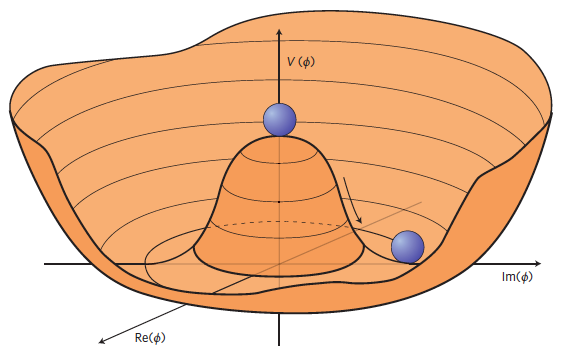
\includegraphics[width= .7\textwidth]{Figures/Introduction/higgspotential.png}
\caption{Form of the Higgs potential giving rise to SSB via the BEH mechanism.}
\label{Figure:Introduction_HiggsPotential}
\end{figure}

\begin{equation}
    \Phi^{\dagger}\Phi = -\frac{\mu^{2}}{2\lambda} = \frac{\nu^2}{2}
\end{equation}

A key constraint to achieve SSB through the BEH mechanism is to ensure that the photon remains massless while the other gauge bosons acquire mass. Hence, the Higgs potential's minimum must correspond to a nonzero VEV exclusively for the neutral scalar field, $\phi^{0}$~\cite{Higgs_VacuumState_Choice}. This condition preserves the $U(1)_{EM}$ symmetry after SSB.

\begin{equation}
    <0|\Phi|0> = \frac{1}{\sqrt{2}} \begin{pmatrix}
        0 \\
        \nu
    \end{pmatrix}
\end{equation}
 
Before expanding the Higgs field around its minimum to study the consequences of SSB, it is important to recall Goldstone's theorem~\cite{Goldstone}, predicting the emergence of a massless scalar (Goldstone) boson after the spontaneous breaking of a continuous symmetry. Out of the four dof introduced by the Higgs field, the three associated with the broken symmetry generators become Goldstone bosons, appearing as massless scalar fields in the Lagrangian. Gauge invariance guarantees that the choice of gauge does not affect the physical predictions of the theory, allowing us to eliminate the Goldstone bosons from the Lagrangian by making an appropriate local gauge transformation. This is referred to as the unitary gauge where the dof associated with the massless Goldstone bosons are replaced with new degrees of freedom corresponding to the longitudinal polarisation states of the gauge bosons ($W^{\pm}/Z$). In the unitary gauge, the Higgs field can be re-expressed as,

\begin{equation}
    \text{BEH} \rightarrow \Phi = \frac{1}{\sqrt{2}}\begin{pmatrix}
        0 \\
        \nu + h
    \end{pmatrix} 
    \label{Equation:Introduction_HiggsField_2}
\end{equation}

where h is the physical Higgs field, the fourth dof in the Higgs sector.

The term in the Lagrangian responsible for generation of the masses of gauge bosons is $(D_\mu\Phi)^\dagger(D^\mu\Phi)$. Substituting Eq.~\ref{Equation:Introduction_HiggsField_2} into this term and expressing the $B_\mu$ and $W_{\mu}^{(i)}$ fields in terms of physical $Z_\mu$ and $W_{\mu}^{\pm}$ states using Eq.~\ref{Equation:Introduction_PhysicalGaugeFields}, we obtain the following weak boson mass terms,

\begin{equation}
    \text{BEH} \rightarrow \mathcal{L}_{\text{Higgs}} \supset \frac{1}{4} g^2 \nu^2 W^{+\mu}W_{\mu}^- + \frac{(g^2+g'^2)\nu^2}{8} Z_\mu Z^\mu
\label{Equation:Introduction_HiggsLagrangian_2}
\end{equation}

Using the known form of a mass term for a spin-1 gauge boson, the masses of the $W^\pm$ and the Z bosons can be expressed in terms of the $SU(2)_{L}$ $\otimes$ $U(1)_{Y}$ gauge couplings and the Higgs VEV ($\nu = 246 \GeV$) as,

\begin{equation}
\begin{array}{c}
    m_W = \frac{1}{2}g\nu \\
    m_Z = \frac{1}{2}\nu\sqrt{g^2+g'^2}\\
\end{array}
\end{equation}

Importantly in this physical basis, the neutral gauge boson associated with the $\text{A}_\mu$ field remains massless while the physical Higgs field also appears in the Lagrangian with the associated terms being,

\begin{equation}
    \text{BEH} \rightarrow \mathcal{L}_{\text{Higgs}} \supset \underbrace{\frac{1}{2} \partial_\mu h \, \partial^\mu h - \lambda \nu^2 h^2}_{\text{massive scalar boson } h}
    \underbrace{- \lambda \nu h^3 - \frac{1}{4} \lambda h^4}_{\text{Higgs self-interactions}}
\label{Equation:Introduction_HiggsLagrangian_3}
\end{equation}

According to Eq.~\ref{Equation:Introduction_HiggsLagrangian_3}, the mass of the scalar boson field in given by $\text{m}_H = \sqrt{2\lambda}\nu$. This Lagrangian also contains terms describing the trilinear and quartic self-interactions of the Higgs boson for which the relevant Feynman diagram are shown in Fig.~\ref{Figure:Introduction_HiggsSelf}. While only the self-interaction terms are shown in Eq.~\ref{Equation:Introduction_HiggsLagrangian_3}, the Lagrangian also contains interactions terms between the Higgs boson and the weak gauge bosons ($W^\pm/Z$). 

\begin{figure}[h]
    \centering
    % First row
    \begin{subfigure}{0.45\textwidth}
        \centering
        \begin{tikzpicture}
    \begin{feynman}
        \vertex[blue] at (0, 0) (a) {\(H\)};
        \vertex at (2, 0) (center);
        \vertex[blue] at (4, 1.5) (b) {\(H\)};
        \vertex[blue] at (4, -1.5) (c) {\(H\)};

        \diagram*{
            (a) -- [scalar] (center),
            (center) -- [scalar] (b),
            (center) -- [scalar] (c),
        };
    \end{feynman}
\end{tikzpicture}


    \end{subfigure}
    \hfill
    \begin{subfigure}{0.45\textwidth}
        \centering
        \begin{tikzpicture}
    \begin{feynman}
        \vertex[blue] at (0, 1.5) (a) {\(H\)};
        \vertex[blue] at (0, -1.5) (a1) {\(H\)};

        \vertex at (2, 0) (center);
        \vertex[blue] at (4, 1.5) (b) {\(H\)};
        \vertex[blue] at (4, -1.5) (c) {\(H\)};

        \diagram*{
            (a) -- [scalar] (center),
            (a1) -- [scalar] (center),
            (center) -- [scalar] (b),
            (center) -- [scalar] (c),
        };
    \end{feynman}
\end{tikzpicture}


    \end{subfigure}
    \caption{Feynman diagrams arising from the presence of the Higgs self-interaction terms in the SM Lagrangian.}
    \label{Figure:Introduction_HiggsSelf}
\end{figure}

Remarkably, fermions in the SM also acquire masses via the Higgs mechanism through Yukawa interactions~\cite{YukawaInteractions}. After SSB, when the Higgs field acquires a VEV, the Yukawa part of the Lagrangian takes the form

\begin{equation}
    \mathcal{L}_{Yukawa}^f = \underbrace{-\frac{g_f}{\sqrt{2}}\nu(\overline{\psi_L}\psi_R + \overline{\psi_R} \psi_L)}_{\text{mass term}} \underbrace{- \frac{g_f}{\sqrt{2}}h(\overline{\psi_L}\psi_R + \overline{\psi_R} \psi_L)}_{\text{interaction term}}
\end{equation}

where $\psi_L$ and $\psi_R$ are the left-handed and right-handed chiral fields, and the first term gives the mass of fermionic mass $m_f = g_f\nu / \sqrt{2}$. The second term in the Lagrangian describes the coupling between the fermion and the Higgs boson itself, interestingly indicating that heavier fermions couple stronger to the Higgs.

\section{The Higgs boson}

Undoubtedly, one of the most significant achievements in modern physics, is the observation of the long-sought fundamental boson, the Higgs. The confirmation of its existence came back in 2012, when the ATLAS and CMS Collaborations~\cite{Higgs_ATLAS,Higgs_CMS} jointly announced its discovery, marking the completion of the SM particle content. Soon after its discovery, both collaborations conducted several measurements exploring the properties of the Higgs, demonstrating that the observed Higgs looks very much alike the SM Higgs~\cite{HiggsParity_1,HiggsParity_2}. One important test lies in the Higgs boson couplings with the most recent measurements of the coupling strengths~\cite{CMS_Couplings_Measurement} being consistent with the SM prediction, as presented in Fig.~\ref{Figure:Introduction_CMScouplings}.

\begin{figure}[h]
\centering
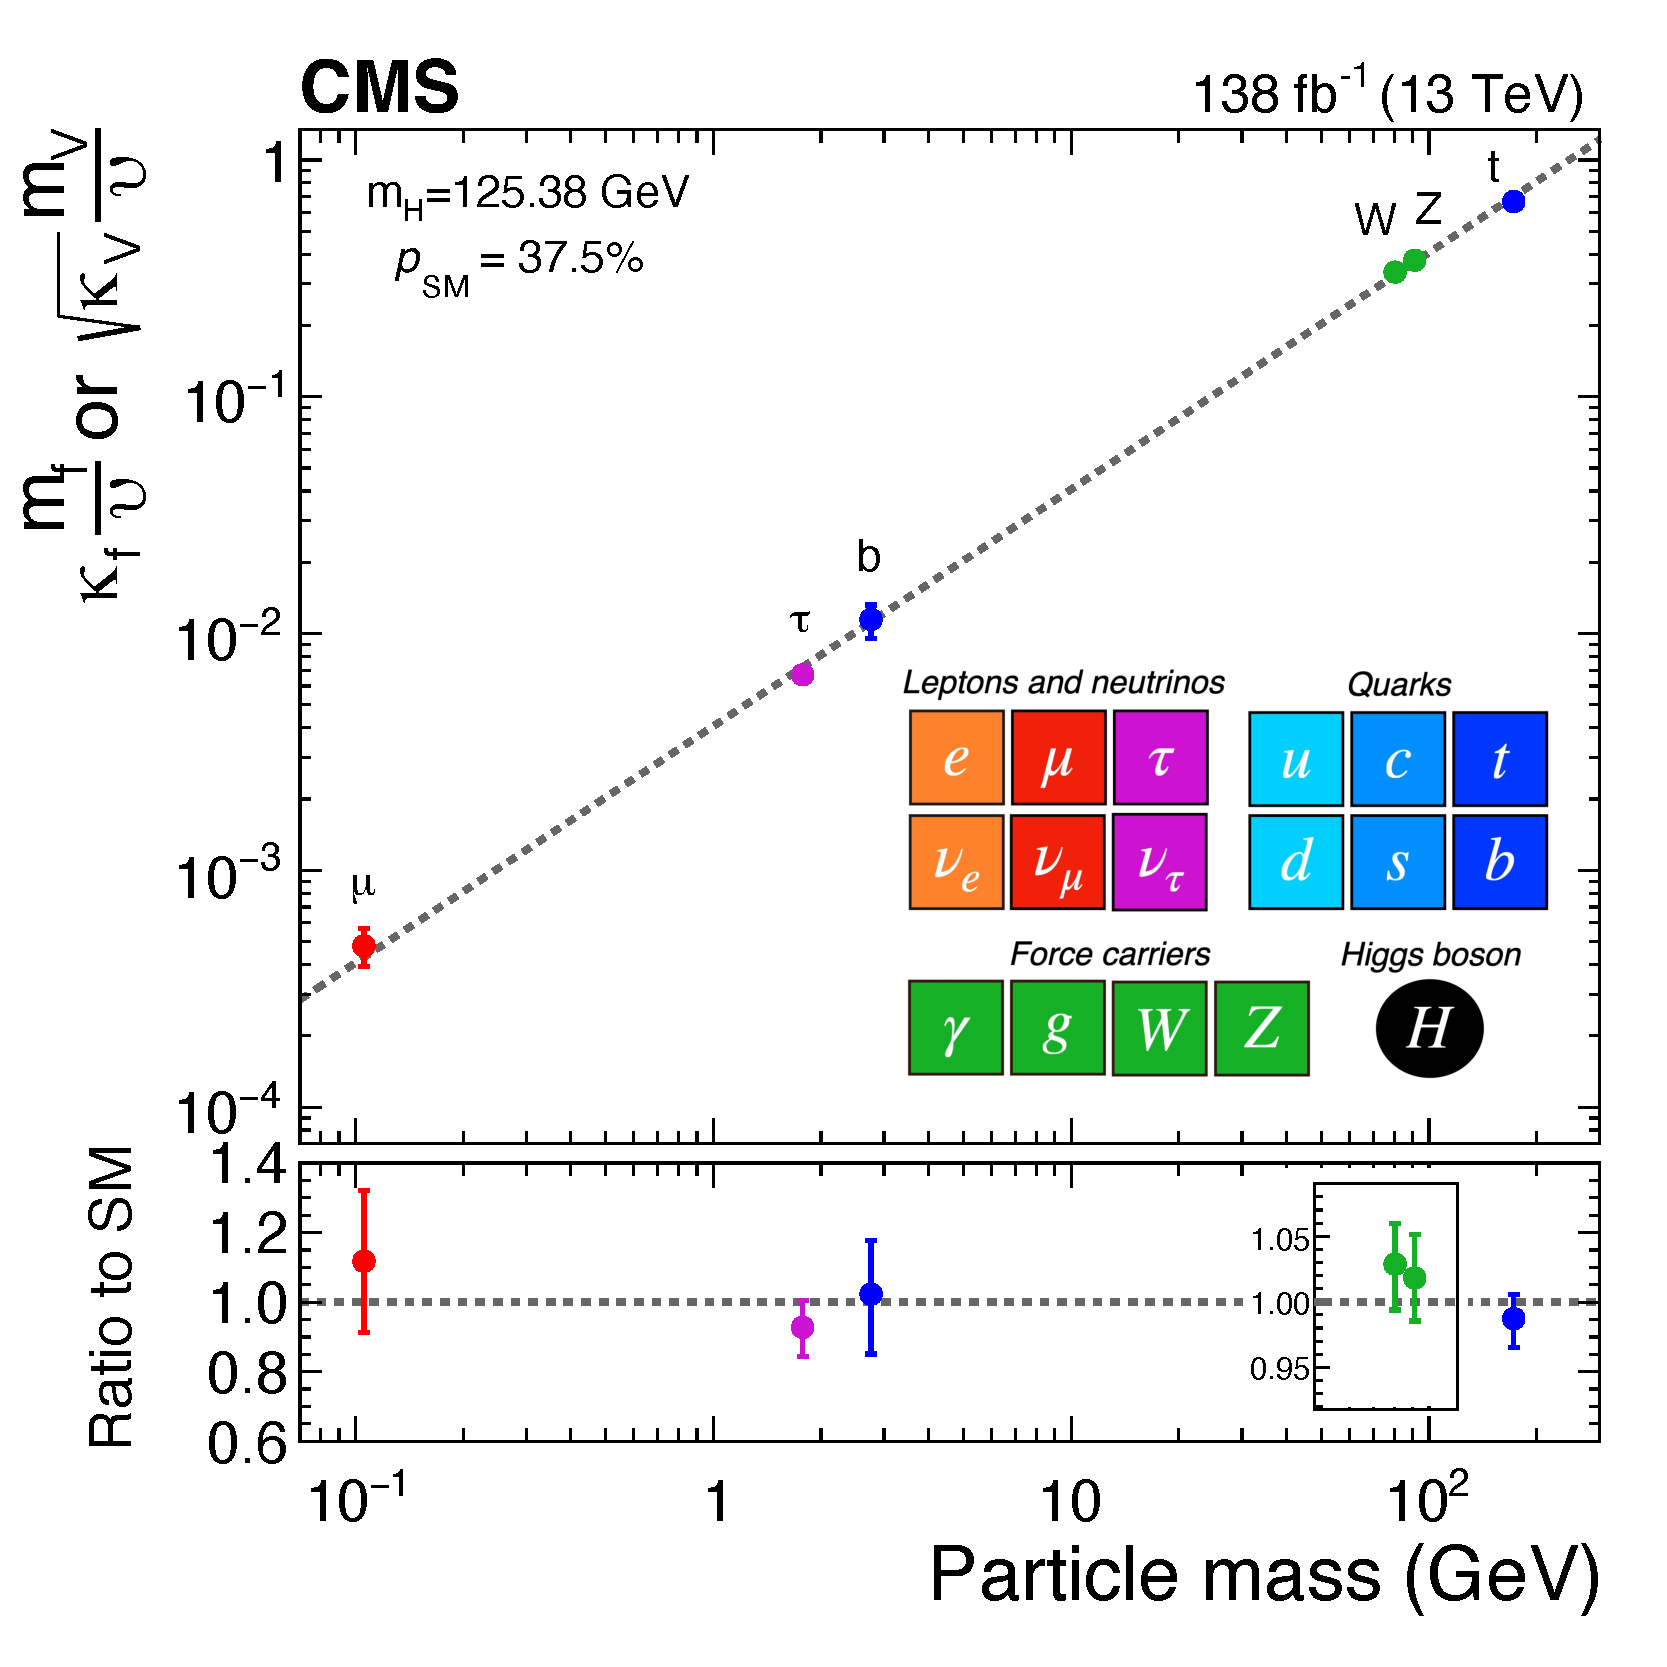
\includegraphics[width= .7\textwidth]{Figures/Introduction/CMS_Higgs_FermionCouplings.pdf}
\caption{The measured coupling strength modifiers of the Higgs boson to fermions and heavy gauge bosons, presented as a function of the fermionic/bosonic masses. For gauge bosons, the "reduced" coupling modifiers are presented, to keep a linear proportionality to the mass~\cite{CMS_Couplings_Measurement}.}
\label{Figure:Introduction_CMScouplings}
\end{figure}

\subsection{Higgs boson production}

At the \ac{LHC}, the Higgs boson is produced via four major production modes; gluon-gluon fusion (ggH), vector boson fusion (VBF), vector boson associated production (VH), and $t\overline{t}$-associated production (ttH); listed in order of decreasing cross-section. In addition to the dominant production modes, the Higgs can still be produced in different ways \eg in association with a single-top (tH). The Feynman diagrams of the dominant modes are displayed in Fig.~\ref{Figure:Introduction_HiggsProductionModes} while their respective cross-sections at $\sqrt{s}$ = 13$\TeV$ and $\sqrt{s}$ = 13.6$\TeV$ are displayed in Table~\ref{Table:Introduction_HiggsProduction_XS}. 


\begin{figure}[h]
    \centering
    % First row
    \begin{subfigure}{0.45\textwidth}
        \centering
        \begin{tikzpicture}
    \begin{feynman}
        \vertex at (0, 1.5) (i1) {\(g\)};
        \vertex at (0,-1.5) (i2) {\(g\)};
        \vertex at (2.5, 1.5) (a);
        \vertex at (2.5,-1.5) (b);
        \vertex at (4, 0) (c);
        \vertex[blue] at (6, 0) (f) {\(H\)};
        \vertex at (3.25,0) () {\(t\)};
        \diagram*{
            (i1) -- [gluon] (a),
            (i2) -- [gluon] (b),
            (a) -- [fermion] (b) -- [fermion] (c) -- [fermion] (a),
            (c) -- [scalar] (f),
        };
    \end{feynman}
\end{tikzpicture}


        \caption{\(ggH\)}
    \end{subfigure}
    \hfill
    \begin{subfigure}{0.45\textwidth}
        \centering
        \begin{tikzpicture}
    \begin{feynman}
        \vertex at (0, 1.) (i1) {\(q\)};
        \vertex at (0,-1.) (i2) {\(q\)};

        \vertex at (3, 1) (a);
        \vertex at (3,-1) (b);
        \vertex at (4,0) (c);

        \vertex[blue] at (6, 0) (f) {\(H\)};
        \vertex at (6, 1.5) (e) {\(q\)};
        \vertex at (6,-1.5) (g) {\(q\)};

        \vertex at (4.25,0.6) () {\(W/Z\)};
        \vertex at (4.25,-0.6) () {\(W/Z\)};

        \diagram*{
            (i1) -- [fermion] (a),
            (i2) -- [fermion] (b),
            (a) -- [photon] (c),
            (b) -- [photon] (c),
            (c) -- [scalar] (f),
            (a) -- [fermion] (e),
            (b) -- [fermion] (g),
        };
    \end{feynman}
\end{tikzpicture}
        \caption{\(VBF\)}
    \end{subfigure}

    % Add vertical space between rows
    \vspace{0.5cm}

    % Second row (centered properly)
    \begin{subfigure}{0.45\textwidth}
        \centering
        \raisebox{-5mm}{\begin{tikzpicture}
    \begin{feynman}
        \vertex at (0, 1.5) (i1) {\(q\)};
        \vertex at (0,-1.5) (i2) {\(\overline{q}\)};

        \vertex at (2,0) (a);
        \vertex at (4, 0) (b);

        \vertex at (6.15, 1.5) (c) {\(W/Z\)};
        \vertex[blue] at (6,-1.5) (d) {\(H\)};

        \vertex at (3,0.25) () {\(W/Z\)};

        \diagram*{
            (i1) -- [fermion] (a) -- [fermion] (i2),
            (a) -- [photon] (b),
            (b) -- [photon] (c),
            (b) -- [scalar] (d),
        };
    \end{feynman}
\end{tikzpicture}}
        \caption{\(WZ\) associated}
    \end{subfigure}
    \hfill
    \begin{subfigure}{0.45\textwidth}
        \centering
        \begin{tikzpicture}
    \begin{feynman}
        \vertex at (0, 1.5) (i1) {\(g\)};
        \vertex at (0,-1.5) (i2) {\(g\)};
        
        \vertex at (3, 1.5) (a);
        \vertex at (3,0) (ab);
        \vertex at (3,-1.5) (b);
        
        \vertex at (6, 1.5) (c) {\(\overline{t}\)};
        \vertex at (6, -1.5) (d) {\(t\)};

        \vertex[blue] at (6, 0) (f) {\(H\)};

        \diagram*{
            (i1) -- [gluon] (a),
            (i2) -- [gluon] (b),
            (c) -- [fermion] (a),
            (a) -- [fermion] (ab),
            (ab) -- [fermion] (b),
            (b) -- [fermion] (d),
            (ab) -- [scalar] (f),
        };
    \end{feynman}
\end{tikzpicture}


        \caption{\(t\bar{t}\) associated}
    \end{subfigure}

    \caption{Feynman diagrams of the main SM Higgs production modes at the LHC.}
    \label{Figure:Introduction_HiggsProductionModes}
\end{figure}


\begin{table}[h]
\centering
\renewcommand{\arraystretch}{1.5} % Increase row height
\arrayrulecolor{black} % Ensure outer border is black
\begin{tabular}{|c|c|c|}
\hline
Mechanism & Cross Section @ 13 TeV [pb] & Cross Section @ 13.6 TeV [pb] \\ \hline \hline 
ggH                                & 48.6  & 52.23 \\ 
\arrayrulecolor{lightgray} \hline
VBF                                & 3.78  & 4.078 \\ 
\arrayrulecolor{lightgray} \hline
WH                                 & 1.37  & 1.457 \\ 
\arrayrulecolor{lightgray} \hline
ZH                                 & 0.76  & 0.9439 \\ 
\arrayrulecolor{lightgray} \hline
ttH                                & 0.51  & 0.57 \\ 
\arrayrulecolor{black} \hline
\end{tabular}
\caption{Cross sections of the dominant Higgs production mechanisms in the SM. Derived for $\text{m}_H = 125\GeV$ and presented for both $\sqrt{\sigma}=13\TeV$ and $\sqrt{\sigma}=13.6\TeV$~\cite{HiggsProduction_XS}.}
\label{Table:Introduction_HiggsProduction_XS}
\end{table}

The ggH production mode is clearly the most dominant one proceeding via an internal quark loop, consequence of the Higgs not directly coupling to the gluon. Despite its dominance, other production modes such as VBF have an interesting feature, additional objects in their final states. These distinct topologies can be leveraged to reduce backgrounds. In particular, the VBF production mode is characterised by two additional energetic jets which tend to have a large spatial separation and a high invariant mass.

\subsection{Higgs boson decays}

The Higgs boson is an unstable particle, decaying almost immediately after its production~\cite{HiggsUnstable}, with its inference only possible from the decay products. The dominant SM Higgs decays channels are listed in Table~\ref{Table:Introduction_HiggsBranchingFractions}, clearly showing that $H\rightarrow b\overline{b}$ is the dominant decay mode. 

\begin{table}[h]
\centering
\renewcommand{\arraystretch}{1.5} % Increase row height
\setlength{\tabcolsep}{12pt} % Increase column width
\arrayrulecolor{black} % Ensure outer border is black
\begin{tabular}{|c|c|}
\hline
Decay Mode                  & Branching Fraction {[}\%{]} \\ \hline \hline
$b\overline{b}$             & 58.24 \\ 
\arrayrulecolor{lightgray} \hline
$WW^*$                      & 21.37 \\ 
\arrayrulecolor{lightgray} \hline
$gg$                        & 8.19  \\ 
\arrayrulecolor{lightgray} \hline
$\tau\tau$                  & 6.27  \\ 
\arrayrulecolor{lightgray} \hline
$c\overline{c}$             & 2.89  \\ 
\arrayrulecolor{lightgray} \hline
$ZZ^*$                      & 2.61  \\ 
\arrayrulecolor{lightgray} \hline
$\gamma\gamma$              & 0.23  \\ 
\arrayrulecolor{lightgray} \hline
$\mu\mu$                    & 0.02  \\ 
\arrayrulecolor{black} \hline
\end{tabular}
\caption{Branching fractions, $\text{B}_f$, of the main SM Higgs boson decay channel for $\text{m}_H = 125\GeV$~\cite{HiggsProduction_XS} where for a particular final state $f$, $\text{B}_f = \Gamma_f/\Gamma_H$, with $\Gamma_f$ and $\Gamma_H$ being the decay width of the final state and the Higgs boson respectively.}
\label{Table:Introduction_HiggsBranchingFractions}
\end{table}

However, the sensitivity of this event is heavily impacted by the presence of large hadronic background. The Higgs discovery was only possible after a combination of several of the decay channels; $H\rightarrow ZZ \rightarrow 4l$, $H\rightarrow \gamma \gamma$, $H\rightarrow WW^*$, $H\rightarrow \tau\tau$ and $H\rightarrow b\overline{b}$, with the di-photon and 4 lepton decay channels being the main contributors. Particularly interesting is the $H\rightarrow \tau\tau$ decay mode, providing a relatively large branching fraction, while being less impaired by backgrounds than $H\rightarrow b\overline{b}$.
